Теория стохастической аппроксимации описывает численные схемы для поиска корня в общем случае неизвестной выпуклой монотонной
функции с несмещенным откликом. Наиболее известным результатом теории стохастической аппроксимации является алгоритм
Роббинса-Монро, задающий численную схему, обеспечивающую сходимость к корню заданного уравнения. В работе \cite{sacks1958asymptotic} показано, что в случае если функции отклика $s$ 
строго выпукла и дважды дифференцируема, то асимптотическая скорость сходимости линейна $\mathcal{O}(\frac{1}{n})$ 

\textit{Определение} \textbf{Стохастическая аппроксимация} --- метод решения задач статистического оценивания,
строящихся в виде последовательного приближения на основании наблюдений, представленных случайной величиной.

\textit{\textbf{Теорема.} Алгоритм Роббинса-Монро}. Алгоритм, выполняющий пересчет по 
правилу $d_{n+1} =d _n + a_d(s^*-s)$ сходится в $L^2$ норме при выполнении:
 \begin{enumerate}
    \item значения функции отклика монотонны и $s$ ограничены: $\exists N\ \forall x : | s(x) | \le N$;
    \item $\sum_{t=0}^\infty a_t = \infty$;
    \item $\exists M : |\sum_{t=0}^\infty a_t^2 |< M$.
\end{enumerate}
\textit{Доказательство:} \label{monro}
Следуя доказательству \cite{blum1954approximation}, используем рекуррентную схема связи между ошибками 
на каждом шаге алгоритма $\gamma_t = d_t - d^*$. 
В этом случае правило обновления Роббинса-Монро запишется как: 
\begin{equation}
    \gamma_n^2 = \mathrm{E_{x_t \sim p(x|s(d))}}(d_n+a_t(s^*-x_t) -d^*)^2.
\end{equation}
Раскрываем квадрат разности:
\begin{equation}
    \gamma_n^2 = (d_n - d^*)^2 + a_t^2 \mathrm{E_{x_t \sim p(x|s(d))}} (s^*-x_t)^2 - 2 a_t \mathrm{E_{x_t \sim p(x|s(d))}}\left[ (s^*-x_t)(d_n-d^*) \right].
\end{equation}
Используем несмещенность оценки $\mathrm{E}_{x \sim p(x|s)} x = s$:
\begin{equation}
    d_n =2 a_t (s^* -s(d))(d_n-d^*).
\end{equation}
Получаем связь между ошибками на каждом шаге $gamma_n$:
\begin{equation}
    \lim_{n \rightarrow \infty} \gamma_n = \gamma_1 + \sum_{j=1}^\infty a_n^2 c_n -2 \sum_1^{\infty} a_n d_n < \infty.
\end{equation}
Сходимость обоснуем через два последовательных шага: \begin{itemize}
    \item  $\sum_{j=1}^\infty a_n^2 c_n < \infty$ , поскольку при $\sum_{j=1} a_n^2 < \infty $ и $c_n$-ограничены;
    \item $\sum_{j=1}^\infty a_n d_n < \sum_{j=1}^\infty a_n^2 c_n$,  т.к $b_n \ge 0$.
\end{itemize}
Покажем, что $\lim_{n \rightarrow \infty}{\gamma_n}=0$ следует из $\sum_{j=1}^\infty a_j  =\infty$ .
Действительно, зададим ряд $m_n = \frac{\gamma_n}{d_n}$, т.к. он неотрицателен, то $\sum_{i=1}^{\infty} a_n k_n = \infty $. 
Тогда $\sum_{i=1}^{\infty} a_n k_n \gamma_N < \infty $. 
Из сходимости ряда из неотрицательных элементов следует, что $\lim_{n \rightarrow \infty} \gamma_n =0$.
$\blacksquare$

Выбор коэффициента $a_n$ в численной схеме существенно влияет на число шагов, необходимых для того, 
чтобы последовательность сошлась. Авторы оригинального алгоритма предлагают в качестве $a_n = \frac{\lambda}{n}$, где коэффициент $\lambda$ определяется 
экспериментально для каждой постановки. Это обстоятельство затрудняет адаптацию метода в практических случаях, поэтому
существуют модификации схемы, не требующие подбора гиперпараметра. Например, в работе \cite{lai1979adaptive}
был разработан метод выбора коэффициентов исходя из требований несмещенности оценки $\mathrm{E}d_n=d$ и 
минимизации дисперсии $\mathbf{D} d_n=0$ на каждом шаге. Такой подход позволил получить оптимальные 
численные коэффициенты для случая цепи гауссовых распределений \cite{liu2024robbins}.

Для ускорения сходимости современные исследователи дополняют оригинальную схему заменой члена 
$s^*$ на параметр шага $b_n$: $x_{n+1} = x_n - a_n(y_n -b_n)$ \cite{krasulina2007}. Доказательство сходимости метода описано в работе \cite{joseph2004efficient}.

\textit{\textbf{Теорема.} Алгоритм Роббинса-Монро для случая $b_n \ne s^*$}  \cite{joseph2004efficient} Модифицированная схема $x_{n+1} = x_n - a_n(y_n -b_n)$ сходится
в условиям сходимости алгоритма Роббинса-Монро при условии:
\begin{equation}
    \sum_{n=2}^\infty a_n |b_n - s^*| \sum_{j=1}^{n-1} a_j < \infty \
\end{equation}
% \textit{Доказательство}:

% Принципиальная схема доказательства значительно не изменяется
% \begin{equation}
%     (d_n - d^*)^2 + a_t^2 \mathrm{E_{x_t \sim p(x|s(d))}} (b_t-x_t)^2 - 2 a_t \mathrm{E_{x_t \sim p(x|s(d))}}\left[ (b_t-x_t)(d_n-d^*) \right].
% \end{equation}

% $\blacksquare$
На практике также представляет интерес работы с многомерными данными. В работе \cite{xiong2018efficient} описан подход с вектором бинарных величин.

\textit{\textbf{Теорема.} Алгоритм Роббинса-Монро для многомерного бинарного случая} \cite{xiong2018efficient}:
 Пусть $\mathbf{x}$ --- вектор бернулевских случайных величин с параметрами $\mathbf{s}=f(\mathbf{d})$, 
 где $f(\mathbf{x})$ --- выпуклая.
 Тогда схема пересчета $d_t=\mathbf{x}_t + A^{(t)} (s - \mathbf{x}_t)$ с шагами $A^{(t)}$, удовлетворяющими условиям:
 $\forall t,j \rightarrow a_{jj}^{(t)} >0,
 \sum^{\infty}_{t=1} a_{jj}^{(t)} = \infty,
  \sum_{n=1}^\infty (a^{(t)}_{jj})^2 < \infty$
сходится по вероятности к целевому значению $\mathbf{s}^*$

\textbf{Доказательство:} 
\begin{equation}
    \begin{aligned}
        & \mathrm{E}\left\{\left(\mathbf{x}_{n+1}-\boldsymbol{\theta}\right)^{\top}\left(\mathbf{x}_{n+1}-\boldsymbol{\theta}\right)\right\} \\
        & \quad=\mathrm{E}\left(\mathrm { E } \left[\left\{\mathbf{x}_{n}-\boldsymbol{\theta}-A_{n}\left(\mathbf{y}_{n}-\boldsymbol{\alpha}\right)\right\}^{\top}\right.\right. \\
        & \left.\left.\quad \times\left\{\mathbf{x}_{n}-\boldsymbol{\theta}-A_{n}\left(\mathbf{y}_{n}-\boldsymbol{\alpha}\right)\right\} \mid \mathbf{x}_{n}\right]\right) \\
        & \quad=\mathrm{E}\left(\mathbf{x}_{n}-\boldsymbol{\theta}\right)^{\top}\left(\mathbf{x}_{n}-\boldsymbol{\theta}\right)-2 \mathrm{E}\left(\mathbf{x}_{n}-\boldsymbol{\theta}\right)^{\top} A_{n}\left(\mathbf{m}_{n}^{x}-\boldsymbol{\alpha}\right) \\
        & \quad+\mathrm{E}\left\{\left(\mathbf{y}_{n}-\boldsymbol{\alpha}\right)^{\top} A_{n}^{\top} A_{n}\left(\mathbf{y}_{n}-\boldsymbol{\alpha}\right)\right\} \\
        & \quad=\mathrm{E}\left(\mathbf{x}_{1}-\boldsymbol{\theta}\right)^{\top}\left(\mathbf{x}_{1}-\boldsymbol{\theta}\right)-2 \sum_{i=1}^{n} \mathrm{E}\left(\mathbf{x}_{i}-\boldsymbol{\theta}\right)^{\top} A_{i}\left(\mathbf{m}_{i}^{x}-\boldsymbol{\alpha}\right) \\
        & \quad+\sum_{i=1}^{n} \mathrm{E}\left\{\left(\mathbf{y}_{i}-\boldsymbol{\alpha}\right)^{\top} A_{i}^{\top} A_{i}\left(\mathbf{y}_{i}-\boldsymbol{\alpha}\right)\right\} \\
        & \quad \geq 0,
    \end{aligned} 
\end{equation}
где ожидания получены по $\mathbf{x}_{n}, \mathbf{m}_{n}^{x}=
\mathrm{E}\left(\mathbf{y}_{n} \mid \mathbf{x}_{n}\right)=\left(M_{1}\left(x_{1 n}\right),
\ldots, M_{p}\left(x_{p n}\right)\right)^{\top}$.
 
Обозначим $\mathbf{e}_{i}=\left(e_{11}, \ldots,e_{p i}\right)^{\top}=\mathbf{y}_{i}-\boldsymbol{\alpha}$. 
Из ограниченности $e_{j i}$ сумма $\sum_{i=1}^{n} \mathrm{E}\left\{\left(\mathbf{y}_{i}-\boldsymbol{\alpha}\right)^{\top} A_{i}^{\top} A_{i}\left(\mathbf{y}_{i}-\boldsymbol{\alpha}\right)\right\}$ запишется как 

$\sum_{j=1}^{p} \sum_{i=1}^{n}\left\{\mathrm{E}\left(e_{j i}^{2}\right) \sum_{s=1}^{p} a_{s j, i}^{2}\right\}+\sum_{j \neq k} \sum_{i=1}^{n}\left\{\mathrm{E}\left(e_{j i} e_{k i}\right) \sum_{s=1}^{p} a_{s j, i} a_{s k, i}\right\}$.

Докажем в два шага:
 \begin{enumerate}
    \item Ряды $\sum_{i=1}^{n}\left\{\mathrm{E}\left(e_{j i}^{2}\right) \sum_{s=1}^{p} a_{s j, i}^{2}\right\}$ 
    и $\sum_{i=1}^{n}\left\{\mathrm{E}\left(e_{j i} e_{k i}\right) \sum_{s=1}^{p} a_{s j, i} a_{s k, i}\right\}$ 
    сходятся. Следовательно, сходится и ряд 
    $\sum_{i=1}^{n} \mathrm{E}\left\{\left(\mathbf{y}_{i}-\boldsymbol{\alpha}\right)^{\top} A_{i}^{\top} A_{i}\left(\mathbf{y}_{i}-\boldsymbol{\alpha}\right)\right\}$
    , причем к положительному значению $\sum_{n=1}^{\infty} \mathrm{E}\left\{\mathbf{x}_{n}-\boldsymbol{\theta}^{\top} A_{n}\left(\mathbf{m}_{n}^{x}-\boldsymbol{\alpha}\right)\right\}<\infty$.
    \item Также для $j=1, \ldots, p$, поскольку $M_{j}$ функция распределения и 
    $\dot{M}_{j}\left(\theta_{j}\right)>0$, существует положительные постоянные $\ell_{j}$ и $u_{j}$ такие что:
    $$
        0<\ell_{j} \leq \frac{M_{j}\left(x_{j}\right)-\alpha_{j}}{x_{j}-\theta_{j}} \leq u_{j}<\infty
    $$
    для всех $x_{j}$. Пусть $\ell=\min \left\{\ell_{j}: j=1, \ldots, p\right\}$ и $u=\max \left\{u_{j}: j=\right.$ $1, \ldots, p\}$. 
\end{enumerate}
Обозначим $\mathbf{a}_{j, n}$ $j$ столбцом матрицы $A_{n}$. Тогда:
\begin{equation}
    \begin{aligned}
        & \left(\mathbf{x}_{n}-\boldsymbol{\theta}\right)^{\top} A_{n}\left(\mathbf{m}_{n}^{x}-\boldsymbol{\alpha}\right) \\
        & =\sum_{j=1}^{p}\left(\mathbf{x}_{n}-\boldsymbol{\theta}\right)^{\top} \mathbf{a}_{j, n}\left(x_{j n}-\theta_{j}\right) \frac{M_{j}\left(x_{j n}\right)-\alpha_{j}}{x_{j n}-\theta_{j}} \\
        & \geq \sum_{j=1}^{p}\left(\mathbf{x}_{n}-\boldsymbol{\theta}\right)^{\top} \mathbf{a}_{j, n}\left(x_{j n}-\theta_{j}\right) \delta_{j n} \\
        & =\left(\mathbf{x}_{n}-\theta\right)^{\top} A_{n} \Delta_{n}\left(\mathbf{x}_{n}-\theta\right),
    \end{aligned}
\end{equation}
где $\Delta_{n}=\operatorname{diag}\left(\delta_{1 n}, \ldots, \delta_{p n}\right)$ с
\begin{equation}
    \delta_{j n}= \begin{cases}
        \ell, & \text{если} \left(\mathbf{x}_{n}-\boldsymbol{\theta}\right)^{\top} \mathbf{a}_{j, n}\left(x_{j n}-\theta_{j}\right) \geq 0  \\
        u,\quad \text{иначе}
    \end{cases}
\end{equation}
Следовательно, имея $\sum_{n=1}^{\infty} \mathrm{E}\left(\mathbf{x}_{n}-\theta\right)^{\top} A_{n} \Delta_{n}\left(\mathbf{x}_{n}-\theta\right)<\infty$. 
Поскольку это выражение можно записать как:
\begin{align*}
    & \sum_{j=1}^{p} \sum_{n=1}^{\infty} a_{j j, n} \delta_{j n} \mathrm{E}\left(x_{j n}-\theta_{j}\right)^{2} \\
    & \quad+\sum_{j \neq k} \sum_{n=1}^{\infty} a_{j k, n} \delta_{k n} \mathrm{E}\left(x_{j n}-\theta_{j}\right)\left(x_{k n}-\theta_{k}\right) \tag{A2}
\end{align*}
Заметим, что для второго члена выполняется:
\begin{equation}
    \begin{aligned}
        & \sum_{j \neq k} \sum_{n=1}^{\infty} \frac{1}{2}\left|a_{j k, n} \delta_{k n}\right|\left\{\mathrm{E}\left(x_{j n}-\theta_{j}\right)^{2}+\mathrm{E}\left(x_{k n}-\theta_{k}\right)^{2}\right\} \\
        & \quad=\frac{1}{2} \sum_{j=1}^{p} \sum_{n=1}^{\infty} \mathrm{E}\left(x_{j n}-\theta_{j}\right)^{2} \sum_{k \neq j}\left\{\left|a_{j k, n} \delta_{k n}\right|+\left|a_{k j, n} \delta_{j n}\right|\right\} .
    \end{aligned}
\end{equation}
Предположение $\left|a_{j k, n} / a_{j j, n}\right| \rightarrow 0$ где $n \rightarrow \infty$ для $j \neq k$ и $a_{j j, n}>0$
означает, что $\exists N: \forall n>N,\left|a_{j k, n}\right|<a_{j j, n} /\{2 c(p-1)\}, k \neq j$, 
где $c$ константа большая $u /(2 \ell)$ и $u$ и $\ell$ . Тогда для заданного $j$ выполняется:
\begin{equation}
    \begin{aligned}
        & \sum_{k \neq j}\left|a_{j k, n} \delta_{k n}\right|+\left|a_{k j, n} \delta_{j n}\right|<\sum_{k \neq j}\left\{\frac{a_{j j, n} \delta_{k n}}{2 c(p-1)}+\frac{a_{j j, n} \delta_{j n}}{2 c(p-1)}\right\} \\
        & \quad<\frac{a_{j j, n} u}{c}
    \end{aligned}  
\end{equation}
Тогда сумма запишется как:
\begin{equation}
    \begin{aligned}
        & \sum_{j=1}^{p} \sum_{n>N}^{\infty} a_{j j, n} \delta_{j n} \mathrm{E}\left(x_{j n}-\theta_{j}\right)^{2} \\
        & +\sum_{j \neq k} \sum_{n>N}^{\infty} a_{j k, n} \delta_{k n} \mathrm{E}\left(x_{j n}-\theta_{j}\right)\left(x_{k n}-\theta_{k}\right) \\
        &  \geq \sum_{j=1}^{p} \sum_{n>N}^{\infty} a_{j j, n} \delta_{j n} \mathrm{E}\left(x_{j n}-\theta_{j}\right)^{2}-\frac{1}{2} \sum_{j=1}^{p} \sum_{n>N}^{\infty} \mathrm{E}\left(x_{j n}-\theta_{j}\right)^{2} \\
        &  \times \sum_{k \neq j}\left\{\left|a_{j k, n} \delta_{k n}\right|+\left|a_{k j, n} \delta_{j n}\right|\right\} \\
        & >\sum_{j=1}^{p} \sum_{n>N}^{\infty}\left(\delta_{j n}-\frac{u}{2 c}\right) a_{j j, n} \mathrm{E}\left(x_{j n}-\theta_{j}\right)^{2}
    \end{aligned}
\end{equation}
Заметим, что оценка положительна исходя из выбора $c$. Следовательно, исходя из $\mathrm{E}\left(x_{j n}-\theta_{j}\right)^{2}$ сходится к 0 $\forall j= 1, \ldots, p$,
что означает сходимость по вероятности последовательности $\mathbf{x}_{n}$ к $\boldsymbol{\theta}$
$\blacksquare$

Стохастическую аппроксимацию можно представить
как непрерывную постановку $\dot{z} = g(z(t))$. Для этого запишем численную схему в более общем виде:
\begin{equation}
    x_{n+1} = x_n + a_n \left[g(x_n) + \varepsilon_n \right],
\end{equation}
где $g(x_n)$ --- преобразование, сужающее ряд к решению $x^*$. Зададим промежутки наблюдения $t_n$ через шаги $a_n$:
\begin{equation}
    t_n = \sum_{k=0}^n a_k 
\end{equation}
Заметим, что в условиях сходимости алгоритма Роббинса-Монро, последовательность времен неограничена, 
т.к. $\sum_{k=0}^n a_k =\infty$.
Но шаг с течением времени сужается как $\frac{1}{n^2}$ в асимптотике $\sum_{k=0}^n a^2_k < \infty$. 
Покажем, что в условиях липшицевости $g(x_t)$ существует аппроксимирующее схему обыкновенное дифференциальное уравнение.

\begin{figure}[h]
    \centering
    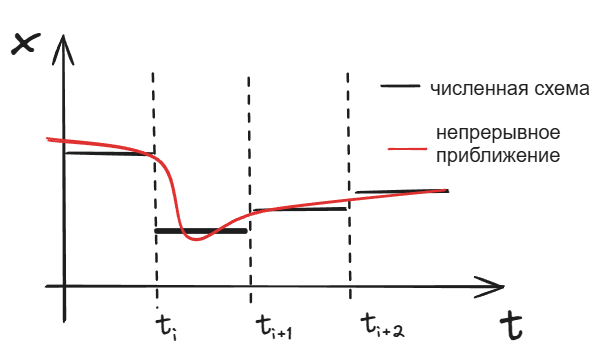
\includegraphics[width=0.5\textwidth]{assets/math/approx/cont_vs_discrete.excalidraw.png}
    \caption{Численная схема стохастической аппроксимации может быть приближена дифференциальным уравнением $\frac{d z}{d t} = g(z(t))$ }
    \label{continuiation}
\end{figure}

\textit{\textbf{Теорема:} Об переходе к непрерывному случаю} Обыкновенное дифференциальное уравнения $\frac{d z_m}{d t} = g(z_m(t))$ c начальным условиями $z(t_m )=x_m$ аксиоматически аппроксимирует
численную схему вблизи бесконечности $x_{n+1} = x_n + a_n \left[g(x_n) + \varepsilon_n \right]$:
$$
    \lim_{m \rightarrow \infty} \sup_{t \in [t_m, t_{m+1} ] } |x(t) - z_m(t)|=0, 
$$
при условиях липшицевости сужающей функции  $\exists L \forall x,y: |g(x) - g(y)| < L |x-y|$.

\textit{Доказательство:} Для доказательства утверждения рассмотрим связь между интегральной формой дифференциального уравнения и численной
аппроксимацией алгоритма. Для этого запишем заданное дифференциальное уравнение в интегральной форме:
\begin{equation}
    z(t_m) = z(t_n) + \int_{t_m}^{t_n} z_m(u)du
    \label{cont_ode}
\end{equation}
Стохастический ряд приближений согласно алгоритму Роббинса-Монро запишется как:
\begin{equation}
    x(t_n) = x_m + \sum{k=m} a_k g(x_k) + \sum_{k=m}^{n-1} a_k \varepsilon_k 
\end{equation}
С учетом \ref{cont_ode} и  $z(t_m)=x_m$:
\begin{equation}
    x(t_n) = x_m + \int_{t_m}^{t_n} g(x([u]_a)) + \sum_{k=m}^{n-1} a_k \varepsilon_k, 
\end{equation}
где $[u]_a$ ступенчатая функция $\max_k(k: t_k \le u)$. 

Рассмотрим искомое выражение как разность полученных представлений:
\begin{equation}
    \| z(t_n) - x(t_n) \| \le \|\sum_{k=m}^{n-1} a_k \varepsilon_k \|+ \int_{t_m}^{t_n} \|g(z(u)) - g([u]_a)\|
\end{equation}
Воспользуемся липшицевостью функции $g(z)$:
\begin{equation}
    \| z(t_n) - x(t_n) \| \le  \|\sum_{k=m}^{n-1} a_k \varepsilon_k \| + L \int_{t_m}^{t_n} |z(u) - x([u_a])|du 
\end{equation}
Используем лемму Гронуолла для перехода к произведению вида:
\begin{equation}
    \| z(t_n) - x(t_n) \| \le  С \|\sum_{k=m}^{n-1} a_k \varepsilon_k \| exp(L \int_{t_m}^{t_n} du) \le C \|\sum_{k=m}^{n-1} a_k \varepsilon_k \| exp(L (t_n -t_m)),
\end{equation}
где $C$ --- положительные константы.
Оценим сверху ряд $\sum_{k=m}^{n-1} a_k \varepsilon_k$ используя аддитивность матожидания:
\begin{equation}
    \| \sum_{k=m}^{n-1} a_k \varepsilon_k \| \le \sum_{k=1}^n a_k \mathrm{E} \varepsilon_k^2 \le \sigma^2 \sum^\infty_{k=1} a_k^2 \le \infty  
\end{equation}
Тогда в силу ограниченности заданного ряда получим:
\begin{equation}
    \lim_{t_n - t_m \rightarrow 0} \| z(t_n) - x(t_n) \|  = 0 
\end{equation}
Или, что эквивалентно:
\begin{equation}
    \lim_{m \rightarrow \infty} \sup_{t \in [t_m, t_{m+1} ] } |x(t) - z_m(t)|=0, 
\end{equation}
$\blacksquare$

Существенный вклад в развитие методов стохастической аппроксимации внёс Б. Т. Поляк \cite{polyak1990new},
предложивший метод усреднения управляющего параметра $\theta$:
 \begin{equation}
     \hat{\theta}_{n+1} = \sum_{i=0}^n \theta_i.
     \label{polyak}
 \end{equation}
Такой подход позволяет подавлять высокочастотные шумовые компоненты при аппроксимации ряда, что позволяет использовать 
методы с большим шагом спуска. Условия эффективной применимости состоят в малом изменении коэффициентов $a_n$:
 \begin{equation}
    \frac{a_{n}-a_{n+1}}{a_{n}}=\mathit{o}(a_{n}).
    \label{polyak_assumptions}
 \end{equation}

% Заданный момент имеет скорость сходимости $\mathcal{O}(\frac{1}{\sqrt{n}})$ для произвольной выпуклой функции. 

% Зададим через $\sigma = \mathbf{E}\left[\nabla f(x_*,\xi)\nabla f(x_*, \xi)^T\right]$ матрицу Гессе в точке сходимости:
% \begin{equation}
%     (\hat{x}^N - x_*) \rightarrow \mathcal{N}(0,\sigma^2)
% \end{equation}

% Схема Стохастической аппроксимации Поляка-Руперта-Юдицкого, изложенная в работе Робинсона и 
% Монро \cite{robbins1951stochastic}:
% \begin{equation}
%     x^{k+1} = x^{k} - \gamma_k \phi(\nabla_x f(x^k,\xi^k))
% \end{equation}
% Шаги $h_k \sim k^{-\alpha}$, $\alpha in (\frac{1}{2},1)$.
% При этом ошибка рассчитывается для среднего
% \begin{equation}
%     \bar{x_n} = \frac{1}{N} \sum_{k=1} x^k
% \end{equation}



